\documentclass{article}

\usepackage{pgfplots}
\pgfplotsset{compat=1.10}

\begin{document}
\makeatletter
\fbox{%
		\tikzpicture
			\pgfplotsplothandlermesh@defaultlegend@img{%
				/pgfplots/shader=interp,
				% undo some shift hard-coded in the macro:
				%yshift=0.7cm,%
				%
				% this repairs it!
				%scale=1/0.4,
			}%
		\endtikzpicture
}%

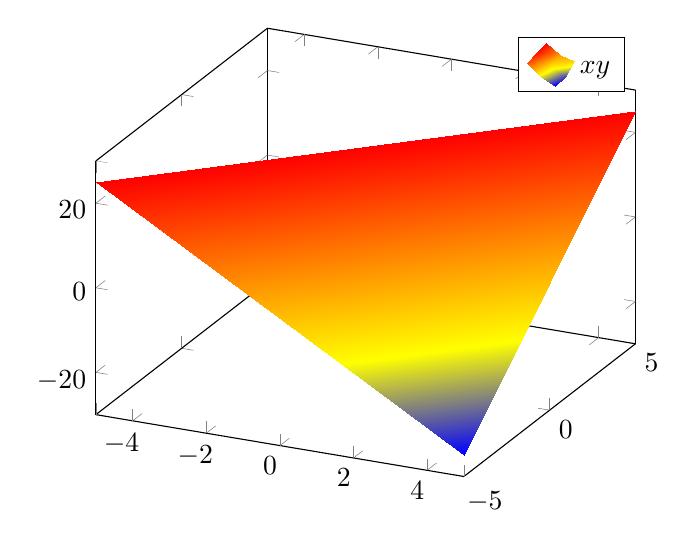
\begin{tikzpicture}
	\begin{axis}[legend entries=$xy$]
	\addplot3[surf,samples=2,shader=interp] {x*y};
	\end{axis}
\end{tikzpicture}

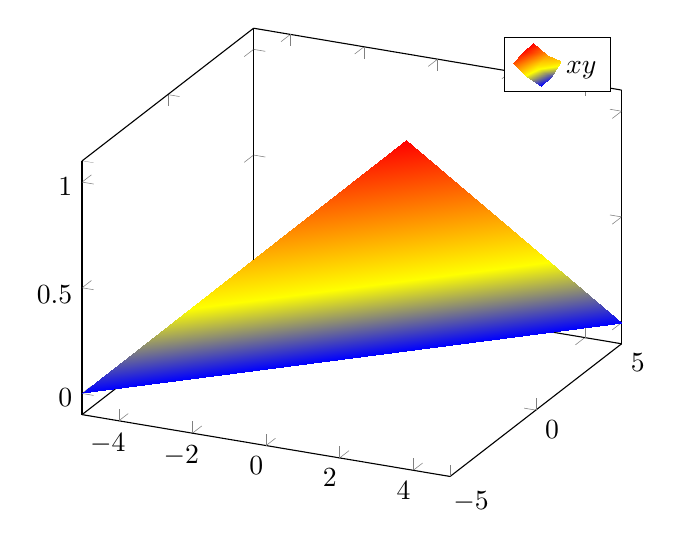
\begin{tikzpicture}
	\begin{axis}[legend entries=$xy$]
	\addplot3[patch,samples=2,patch type=triangle,shader=interp] table {
		-5 -5 0
		5 5 0
		1 1 1
	};
	\end{axis}
\end{tikzpicture}

\fbox{%
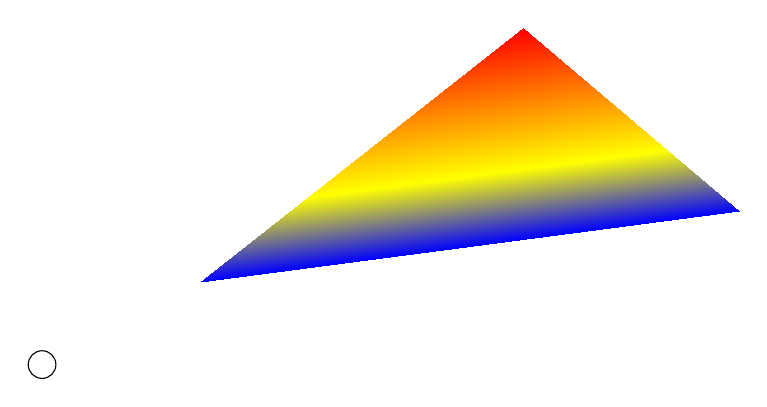
\begin{tikzpicture}
	\begin{axis}[hide axis,clip=false]
	\addplot3[patch,xshift=2cm,samples=2,patch type=triangle,shader=interp] table[row sep=\\] {
		-5 -5 0\\
		5 5 0\\
		1 1 1\\
	};
	\end{axis}
	\draw (0,0) circle (5pt);
\end{tikzpicture}}
\end{document}
